\clearpage%if the chapter heading starts close to bottom of the page, force a line break and remove the vertical vspace
%\vspace{21.5pt}


\chapter{Theoretical background}\label{ch:theoretical-background}

The following sections will detail relevant background concerning malicious network traffic, \gls{ids} workings, and supervised machine learning methods.
The chosen types of malicious network traffic and their descriptions will be detailed.
Furthermore, a brief explanation of \gls{ids}, its classes and methods of detection will be described.
In the same manner, a few selected machine learning algorithms that are useful in classification problems will be briefly explained.

\section{Malicious Network Traffic}\label{sec:malicious-network-traffic}

Malicious network traffic is any network traffic that is intended to harm or breach information systems without the consent of their owners.
As an example, The United States of America's Computer Fraud and Abuse Act (CFAA) bill includes this in a more expansive definition to include cause of damage in monetary form, loss of data, modification of data, extortion, physical, death or otherwise~\cite{code20201030}.
General examples of malicious network traffic include \gls{DoS} attacks, phishing, malware delivery, and ransomware among others.
In the context of this thesis, the following cyberattacks are considered in the implemented solution: code injection specifically \gls{sql} injection, command injection, \gls{xss}, \gls{DoS} attacks, and brute force attacks.

\subsection{SQL Injection}\label{subsec:sql-injection}

Code injection is a method to input code in an application that was not meant to be executed by that application~\cite{Mitropoulos2011}.
As a form of attack it means inputting code that is malicious to be executed by an application.
In a non-attack form, this means adding code that is benign, for instance, adding some extra functionality that is not present in an application.
\gls{sql} injection is a type of code injection where \gls{sql} statements are passed and executed by an application that builds and executes \gls{sql} queries from input passed by a user.
A trivial example of an \gls{sql} injection can be an e-commerce application that contains a form where a user can search for products;
expected input from the application's point of view is input such as ``SD card'' or ``M.2 SSD''.

\begin{code}
    \begin{minted}{sql}
       SELECT * FROM items where items.name = 'SD card'; --normal query
       SELECT * FROM items WHERE items.name = 'SD card'; DROP table items--' --query with injected code
    \end{minted}
\captionof{listing}{\gls{sql} statements showing an \gls{sql} injection}
\label{code:sqlinject}
\end{code}

Assuming in this example that the data is fetched from an \gls{sql} database, the application will build an \gls{sql} query from the user input as shown in listing~\ref{code:sqlinject} line number one.
Without proper input validation in the application, one could pass input such as ``SD card'; DROP table items-\phantom{}-'' resulting in the built query shown in listing~\ref{code:sqlinject} line number two.
The executed query will cause the particular database table to be deleted.

\subsection{Command Injection}\label{subsec:command-injection}
Another type of code injection is command injection.
This differs from \gls{sql} injection in that the extra parsed code is executed by the underlying OS.
Both types of injection are caused by improper validation of user input.

An example of command injection can be an online note application that prior to initializing a writing environment asks for the file name to use;
assuming no validation of user input is done, an attacker could pass extra commands to the underlying OS to be executed, as in
\mintinline{bash}{touch filename ; cat /etc/passwd}.
The extra statement is parsed after the semicolon which indicates that what follows is a sequential command to run.
This could potentially expose sensitive information or grant unauthorized access to the attacker when other commands are passed.

\subsection{Cross-Site Scripting Attack}\label{subsec:xss}
Similarly, \gls{xss} is a type of code injection that allows an attacker to inject malicious code into a vulnerable web application.
It is able to bypass the same origin policy which controls the access of data by and from different domains.
This attack can compromise user data and allow an attacker to perform actions as the compromised-user. \cite{portswigger}

There are three main types of \gls{xss} attacks, namely: reflected, stored, and \gls{dom}-based \gls{xss}.
Reflected \gls{xss} occurs when an attacker injects malicious code into a web request URL, which is then ``reflected'' back to the user when they access the URL.
Stored \gls{xss}, on the other hand, is when the malicious code is stored on the server by an attacker, waiting for unsuspecting users to visit the compromised page.
Finally, \gls{dom}-based \gls{xss} is a type of \gls{xss} that targets the \gls{dom} of a web page.
This type of attack is possible when a web application relies on processing client-side JavaScript to manipulate the \gls{dom}.
If the \gls{dom} can be manipulated by an attacker in this way, they can include malicious code to be run as part of the processing. \cite{portswigger}

\subsection{Denial-of-Service Attack}\label{subsec:dos-attack}
A \gls{DoS} attack is an attack that aims to disrupt the normal functioning of a device or an application service.
The most common case of a \gls{DoS} attack is the disruption of a web service by sending it a flood of requests such that it is unable to contend with the number of requests,
resulting in the service being unavailable or unable to respond to further requests.
It is important to note that a \gls{DoS} attack is launched from a single machine while a \gls{DDoS},
a more advanced form of the same attack, is launched from multiple machines which makes it more difficult to mitigate against.~\cite{cloudflare:denial-of-service}

According to Cloudflare, a \gls{DoS} attack is categorized as either a buffer overflow attack or a flood attack~\cite{cloudflare:denial-of-service}.
In this thesis, an \gls{icmp} ping flood \gls{DoS} attack is used in the implementation of the attack system.
An \gls{icmp} ping flood attack works by sending multiple \gls{icmp} echo requests packets to a target server---if a server is not configured to mitigate against this type of attack, it will reply to each \gls{icmp} echo request packet with a \gls{icmp} echo reply packet thereby consuming resources proportional to the number of requests it received~\cite{cloudflare:ping-flood}.
When the number of requests overwhelms the server's resources, it will result in a \gls{DoS}.


\subsection{Brute Force Attack}\label{subsec:brute-force-attack}

Brute force attack in cybersecurity is a type of attack where an attacker's method of gaining access to a system is to guess and try different combination of passwords through trial-and-error.
In this method the attacker is limited by time, method of guessing, processing power (in case the attack is offline), and possibly any mitigations in the target system.

Due to the advent of powerful GPU hardware technology, the ease of cracking weak passwords has increased dramatically.
If an attacker has access to a hashed password list through any means, they can crack passwords in just a few days with a mid-range GPU.
The suggested mitigation against brute force attacks is to use longer passwords, stronger hashing functions such as bCrypt (a popular hashing function) and perhaps usage of different password schemes such as biometric and graphical passwords.~\cite{ieee:brute-force}

\section{Intrusion Detection System}\label{sec:ids}

An \gls{ids} is a software or hardware system designed to identify and alert on any unauthorized activities that could cause harm to an information system \cite{Khraisat2019}.
They can be broadly categorized into two groups: \gls{sids} and \gls{aids}.
They can also be classified by division into host-based \gls{ids}, network-based \gls{ids}, and hybrid-based \gls{ids} \cite{rajasekaran2012classification};
this latter classification is based on the where the source of data used for analysis is collected from,
more specifically, either from individual devices, a network segment such as a \gls{lan}, or a combination of these.

A \gls{sids} works by having a database of known malicious signatures and it uses those to detect intrusion from collected network traffic or host logs \cites{ieee:ids-classification}{rajasekaran2012classification}{Khraisat2019}.
Due to its method of detection, it can only detect previous flagged signatures and therefore faces significant difficulties in detecting unknown intrusion signatures especially \gls{zero-day} attacks \cite{Khraisat2019}.

On the other hand, \gls{aids} works by defining `normal' behavior of a network and/or computer system by the use of knowledge-based, statistical-based, or machine learning methods; any meaningful deviation from the defined normal behavior is assumed to be an intrusion. \cite{Khraisat2019}.
One advantage of \gls{aids} compared to \gls{sids} is that it can detect previously unseen attacks \cite{rajasekaran2012classification}\cite{ieee:ids-classification}---however, this ability can lead do higher rate of false positive detections due to the threshold of separating malicious and benign behavior \cite{Khraisat2019}.

\section{Supervised Machine Learning Methods}\label{sec:ml-methods}

Supervised machine learning is a type of machine learning that involves training a model on labeled data to predict the output for new, unseen data. In supervised learning, the model is trained using a dataset that contains inputs and their corresponding correct outputs, also known as labels or targets. The goal of the model is then to learn a mapping function between the input and the output, which can then be used for later predictions. \cite{JIANG2020675}

As mentioned previously, the supporting goal of the thesis is to detect whether a particular set of captured traffic is malicious or not;
to achieve this goal, a set of supervised machine learning methods that can be used in classification problems were chosen,
namely---Logistic Regression, \gls{knn}, Random Forest and \gls{mlp}. Note that the selected machine learning methods do not constitute all possible methods that can be used to solve classification problems.

\subsection{K-nearest Neighbors}\label{knn:theory}

\gls{knn} is a non-parametric and lazy learning algorithm that classifies a data point based on its proximity to other data points in a training set.
In this context `lazy learning' means it does not try to learn a general mapping function between inputs and outputs during the training phase, but instead stores the entire training dataset in memory and waits until a new data point is presented to predict it.

Various distance metrics exist to calculate this proximity such as Euclidean distance, Manhattan distance, Hamming distance, and others.
The most popular distance metric is the Euclidean distance which is given by the formula $\sqrt {\sum\nolimits_{i = 1}^n {{{\left( {{x_i} - {y_i}} \right)}^2}} }$ where $x$ and $y$ are respective variables (Eucledian vectors) of data points. \cite{ieee:knn}

An example of how \gls{knn} works visually can be seen in figure \ref{fig:knn}.
The green datapoint is the datapoint that is going to be classified as either belonging to red or blue.

\begin{figure}[ht]
    \centering
    \AltText{A scatter plot showing a dataset with blue and red data points with an additional unlabelled green data point}{\includesvg[width=\textwidth]{knn_example}}
    \caption{\gls{knn} algorithm with a random dataset where the K value is three}
    \label{fig:knn}
\end{figure}

The figure \ref{fig:knn} shows a scatter plot with red and blue labels.
The \gls{knn} algorithm works by calculating the distance metric (Euclidean distance in this case) between the new data point and rest of the data points stored in memory.
From the nearest distance points chosen (three in this case), the label for the new data point is determined to be red if the points are considered to have the same weight (uniform).
On the other hand, the label would be blue if we give closer data points a higher weight than those far away.

Most of the work in \gls{knn} involves choosing the value of K with the help of \gls{cv} to determine the value of K that results in a good test score comparatively.
The base performance of \gls{knn} is determined by the choice of K value, distance metric, and feature scaling. \cite{ieee:knn}


\subsection{Logistic Regression}
Another supervised machine learning method used in classification tasks is Logistic Regression.
It predicts the probability of an input instance belonging to one of two possible classes by applying an activation function to the output of \gls{lr} prediction.

During a Logistic Regression's model training process, \gls{lr} is used to estimate the coefficients that provide the best fit for the input data with respect to the output data;
a sigmoid function---the most common used activation function in Logistic Regression is then used to estimate the probability range between zero and one \cite{ieee:logit}.
Additional activation functions include ReLU, tanh, softmax, and others. An example of a sigmoid function is shown in figure \ref{fig:logit}.

\begin{figure}[H]
    \centering
    \AltText{A probability prediction curve of a logistic regression model with a sigmoid shape (S-shaped)}{\includesvg[width=\textwidth]{logit_example}}
    \caption{An example of logistic regression with a random dataset}
    \label{fig:logit}
\end{figure}

The random dataset in figure \ref{fig:logit} shows a prediction curve for a portion of the dataset set aside as \gls{test-data};
the random data already contains labels zero and one, hence they lie exactly at zero and one in the figure.
For the \gls{test-data}, a prediction is made after training a Logistic Regression model on the \gls{train-data}.
In a binary classification problem, the \gls{decision-threshold} can be chosen to be 0.5 as in this case,
therefore if the probability prediction is greater than 0.5 the output is classified as one and vice-versa.


\subsection{Random Forest}

Random Forest is an \gls{ensemble-method} that makes use of multiple uncorrelated decision trees generated through bagging and feature randomness to make predictions.
In classification tasks, random forests output a prediction based on the majority class encountered in the forest. \cite{ibm:rf}

An example of Random Forest used in a multi-class (more than two) classification is shown in figure \ref{fig:rf}.
In this example, there are four decision trees in the forest.

\begin{figure}[h]
\centering
    \AltText{A diagram showing a random forest constructed from a dataset with four features}{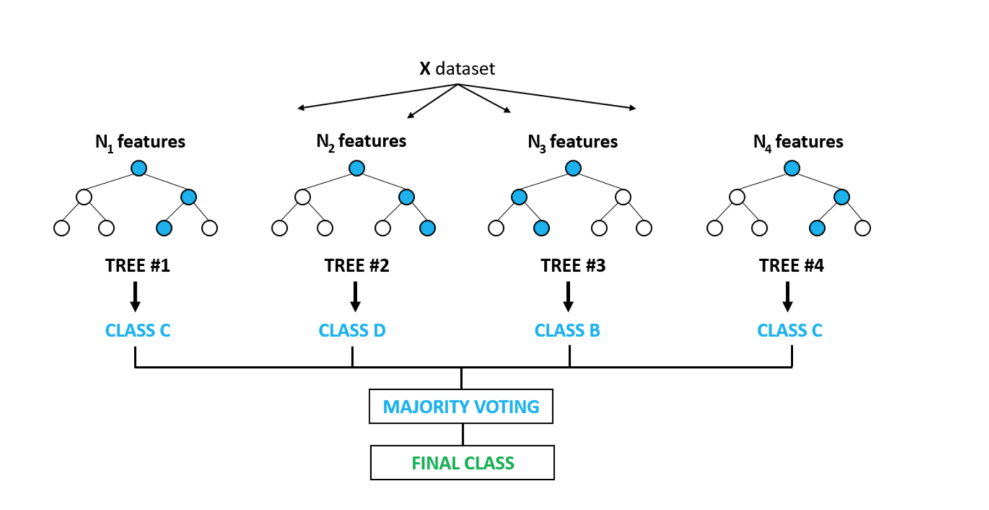
\includegraphics[width=\textwidth]{random-forest}}
    \caption{A Random Forest classification example (Copied from \cite{kirasich2018random})}
    \label{fig:rf}
\end{figure}

In the figure \ref{fig:rf}, the prediction through majority voting is \emph{class C}.
The main benefit purported by Random Forest algorithms include reduced risk of \gls{over-fitting} \cite{ibm:rf} and
resistance to redundant variables \cite{kirasich2018random};
however, they tend to be complex in terms of interpretability \cite{ibm:rf}.

\subsection{Multi-layer Perceptron}

Finally, a \gls{mlp} is a type of \gls{ann} with a feedforward mechanism (outputs are forwarded to the next layer) characterized by
an architecture that consists of an input layer, hidden layer(s), and an output layer;
it additionally makes use of backpropagation to adjust the weights of neurons to minimize the cost function of the output(s). \cite{taud2018multilayer}.


An example of a \gls{mlp} \gls{ann} can be seen in figure \ref{fig:mlp}  with three neurons in the input layer, two neurons in one hidden layer, and one neuron in the output layer.

\begin{figure}[H]
    \centering
    \AltText{A neural network showing neurons that are circular-shaped connected to other neurons in the next layer from left to right}{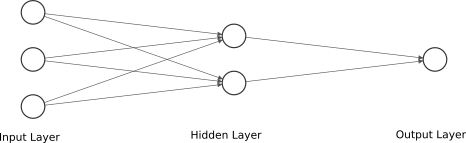
\includegraphics[width=\textwidth]{mlp}}
    \caption{A simple \gls{mlp} \gls{ann} with one hidden layer}
    \label{fig:mlp}
\end{figure}

In the figure \ref{fig:mlp}, the output of the two neurons in the hidden layer are a result of the application of an activation function.
Likewise the output of the neuron in the output layer is also activated---the activation functions used need not be the same in different layers.
Factors such as the number of hidden layers, number of iterations (steps to reduce the cost function), momentum and learning rate have an effect on the performance of a \gls{mlp} model \cite{taud2018multilayer}.
